% Created 2021-03-08 man 18:00
% Intended LaTeX compiler: pdflatex
\documentclass[12pt]{article}

%%%% settings when exporting code %%%% 

\usepackage{listings}
\lstdefinestyle{code-small}{
backgroundcolor=\color{white}, % background color for the code block
basicstyle=\ttfamily\small, % font used to display the code
commentstyle=\color[rgb]{0.5,0,0.5}, % color used to display comments in the code
keywordstyle=\color{black}, % color used to highlight certain words in the code
numberstyle=\ttfamily\tiny\color{gray}, % color used to display the line numbers
rulecolor=\color{black}, % color of the frame
stringstyle=\color[rgb]{0,.5,0},  % color used to display strings in the code
breakatwhitespace=false, % sets if automatic breaks should only happen at whitespace
breaklines=true, % sets automatic line breaking
columns=fullflexible,
frame=single, % adds a frame around the code (non,leftline,topline,bottomline,lines,single,shadowbox)
keepspaces=true, % % keeps spaces in text, useful for keeping indentation of code
literate={~}{$\sim$}{1}, % symbol properly display via latex
numbers=none, % where to put the line-numbers; possible values are (none, left, right)
numbersep=10pt, % how far the line-numbers are from the code
showspaces=false,
showstringspaces=false,
stepnumber=1, % the step between two line-numbers. If it's 1, each line will be numbered
tabsize=1,
xleftmargin=0cm,
emph={anova,apply,class,coef,colnames,colNames,colSums,dim,dcast,for,ggplot,head,if,ifelse,is.na,lapply,list.files,library,logLik,melt,plot,require,rowSums,sapply,setcolorder,setkey,str,summary,tapply},
aboveskip = \medskipamount, % define the space above displayed listings.
belowskip = \medskipamount, % define the space above displayed listings.
lineskip = 0pt} % specifies additional space between lines in listings
\lstset{style=code-small}
%%%% packages %%%%%

\usepackage[utf8]{inputenc}
\usepackage[T1]{fontenc}
\usepackage{lmodern}
\usepackage{textcomp}
\usepackage{color}
\usepackage{graphicx}
\usepackage{grffile}
\usepackage{wrapfig}
\usepackage{rotating}
\usepackage{longtable}
\usepackage{multirow}
\usepackage{multicol}
\usepackage{changes}
\usepackage{pdflscape}
\usepackage{geometry}
\usepackage[normalem]{ulem}
\usepackage{amssymb}
\usepackage{amsmath}
\usepackage{amsfonts}
\usepackage{dsfont}
\usepackage{array}
\usepackage{ifthen}
\usepackage{hyperref}
\usepackage{natbib}
\RequirePackage{setspace} % to modify the space between lines - incompatible with footnote in beamer
\renewcommand{\baselinestretch}{1.1}
\geometry{top=1cm}
\usepackage{titlesec}
\usepackage{etoolbox}
\makeatletter
\patchcmd{\ttlh@hang}{\parindent\z@}{\parindent\z@\leavevmode}{}{}
\patchcmd{\ttlh@hang}{\noindent}{}{}{}
\makeatother
\RequirePackage{colortbl} % arrayrulecolor to mix colors
\definecolor{myorange}{rgb}{1,0.2,0}
\definecolor{mypurple}{rgb}{0.7,0,8}
\definecolor{mycyan}{rgb}{0,0.6,0.6}
\newcommand{\lightblue}{blue!50!white}
\newcommand{\darkblue}{blue!80!black}
\newcommand{\darkgreen}{green!50!black}
\newcommand{\darkred}{red!50!black}
\definecolor{gray}{gray}{0.5}
\hypersetup{
citecolor=[rgb]{0,0.5,0},
urlcolor=[rgb]{0,0,0.5},
linkcolor=[rgb]{0,0,0.5},
}
\newenvironment{comment}{\small \color{gray}\fontfamily{lmtt}\selectfont}{\par}
\newenvironment{activity}{\color{orange}\fontfamily{qzc}\selectfont}{\par}
\RequirePackage{pifont}
\RequirePackage{relsize}
\newcommand{\Cross}{{\raisebox{-0.5ex}%
{\relsize{1.5}\ding{56}}}\hspace{1pt} }
\newcommand{\Valid}{{\raisebox{-0.5ex}%
{\relsize{1.5}\ding{52}}}\hspace{1pt} }
\newcommand{\CrossR}{ \textcolor{red}{\Cross} }
\newcommand{\ValidV}{ \textcolor{green}{\Valid} }
\usepackage{stackengine}
\usepackage{scalerel}
\newcommand\Warning[1][3ex]{%
\renewcommand\stacktype{L}%
\scaleto{\stackon[1.3pt]{\color{red}$\triangle$}{\tiny\bfseries !}}{#1}%
\xspace
}
\newcommand\Rlogo{\textbf{\textsf{R}}\xspace} %
\RequirePackage{fancyvrb}
\DefineVerbatimEnvironment{verbatim}{Verbatim}{fontsize=\small,formatcom = {\color[rgb]{0.5,0,0}}}
\RequirePackage{enumitem} % better than enumerate
\RequirePackage{epstopdf} % to be able to convert .eps to .pdf image files
\RequirePackage{capt-of} %
\RequirePackage{caption} % newlines in graphics
\RequirePackage{tikz-cd} % graph
\RequirePackage{booktabs} % for nice lines in table (e.g. toprule, bottomrule, midrule, cmidrule)
\RequirePackage{amsmath}
\RequirePackage{algorithm}
\RequirePackage[noend]{algpseudocode}
\RequirePackage{dsfont}
\RequirePackage{amsmath,stmaryrd,graphicx}
\RequirePackage{prodint} % product integral symbol (\PRODI)
\usepackage{ifthen}
\usepackage{xifthen}
\usepackage{xargs}
\usepackage{xspace}
\newcommand\defOperator[7]{%
\ifthenelse{\isempty{#2}}{
\ifthenelse{\isempty{#1}}{#7{#3}#4}{#7{#3}#4 \left#5 #1 \right#6}
}{
\ifthenelse{\isempty{#1}}{#7{#3}#4_{#2}}{#7{#3}#4_{#1}\left#5 #2 \right#6}
}
}
\newcommand\defUOperator[5]{%
\ifthenelse{\isempty{#1}}{
#5\left#3 #2 \right#4
}{
\ifthenelse{\isempty{#2}}{\underset{#1}{\operatornamewithlimits{#5}}}{
\underset{#1}{\operatornamewithlimits{#5}}\left#3 #2 \right#4}
}
}
\newcommand{\defBoldVar}[2]{
\ifthenelse{\equal{#2}{T}}{\boldsymbol{#1}}{\mathbf{#1}}
}
\newcommandx\Esp[2][1=,2=]{\defOperator{#1}{#2}{E}{}{\lbrack}{\rbrack}{\mathbb}}
\newcommandx\Prob[2][1=,2=]{\defOperator{#1}{#2}{P}{}{\lbrack}{\rbrack}{\mathbb}}
\newcommandx\Qrob[2][1=,2=]{\defOperator{#1}{#2}{Q}{}{\lbrack}{\rbrack}{\mathbb}}
\newcommandx\Var[2][1=,2=]{\defOperator{#1}{#2}{V}{ar}{\lbrack}{\rbrack}{\mathbb}}
\newcommandx\Cov[2][1=,2=]{\defOperator{#1}{#2}{C}{ov}{\lbrack}{\rbrack}{\mathbb}}
\newcommandx\Binom[2][1=,2=]{\defOperator{#1}{#2}{B}{}{(}{)}{\mathcal}}
\newcommandx\Gaus[2][1=,2=]{\defOperator{#1}{#2}{N}{}{(}{)}{\mathcal}}
\newcommandx\Wishart[2][1=,2=]{\defOperator{#1}{#2}{W}{ishart}{(}{)}{\mathcal}}
\newcommandx\Likelihood[2][1=,2=]{\defOperator{#1}{#2}{L}{}{(}{)}{\mathcal}}
\newcommandx\logLikelihood[2][1=,2=]{\defOperator{#1}{#2}{\ell}{}{(}{)}{}}
\newcommandx\Information[2][1=,2=]{\defOperator{#1}{#2}{I}{}{(}{)}{\mathcal}}
\newcommandx\Score[2][1=,2=]{\defOperator{#1}{#2}{S}{}{(}{)}{\mathcal}}
\newcommandx\Vois[2][1=,2=]{\defOperator{#1}{#2}{V}{}{(}{)}{\mathcal}}
\newcommandx\IF[2][1=,2=]{\defOperator{#1}{#2}{IF}{}{(}{)}{\mathcal}}
\newcommandx\Ind[1][1=]{\defOperator{}{#1}{1}{}{(}{)}{\mathds}}
\newcommandx\Max[2][1=,2=]{\defUOperator{#1}{#2}{(}{)}{min}}
\newcommandx\Min[2][1=,2=]{\defUOperator{#1}{#2}{(}{)}{max}}
\newcommandx\argMax[2][1=,2=]{\defUOperator{#1}{#2}{(}{)}{argmax}}
\newcommandx\argMin[2][1=,2=]{\defUOperator{#1}{#2}{(}{)}{argmin}}
\newcommandx\cvD[2][1=D,2=n \rightarrow \infty]{\xrightarrow[#2]{#1}}
\newcommandx\Hypothesis[2][1=,2=]{
\ifthenelse{\isempty{#1}}{
\mathcal{H}
}{
\ifthenelse{\isempty{#2}}{
\mathcal{H}_{#1}
}{
\mathcal{H}^{(#2)}_{#1}
}
}
}
\newcommandx\dpartial[4][1=,2=,3=,4=\partial]{
\ifthenelse{\isempty{#3}}{
\frac{#4 #1}{#4 #2}
}{
\left.\frac{#4 #1}{#4 #2}\right\rvert_{#3}
}
}
\newcommandx\dTpartial[3][1=,2=,3=]{\dpartial[#1][#2][#3][d]}
\newcommandx\ddpartial[3][1=,2=,3=]{
\ifthenelse{\isempty{#3}}{
\frac{\partial^{2} #1}{\partial #2^2}
}{
\frac{\partial^2 #1}{\partial #2\partial #3}
}
}
\newcommand\Real{\mathbb{R}}
\newcommand\Rational{\mathbb{Q}}
\newcommand\Natural{\mathbb{N}}
\newcommand\trans[1]{{#1}^\intercal}%\newcommand\trans[1]{{\vphantom{#1}}^\top{#1}}
\newcommand{\independent}{\mathrel{\text{\scalebox{1.5}{$\perp\mkern-10mu\perp$}}}}
\newcommand\half{\frac{1}{2}}
\newcommand\normMax[1]{\left|\left|#1\right|\right|_{max}}
\newcommand\normTwo[1]{\left|\left|#1\right|\right|_{2}}
\newcommand\Veta{\boldsymbol{\eta}}
\newcommand\VX{\mathbf{X}}
\author{Brice Ozenne}
\date{\today}
\title{A simple example of multiple imputation using the mice package}
\hypersetup{
 colorlinks=true,
 pdfauthor={Brice Ozenne},
 pdftitle={A simple example of multiple imputation using the mice package},
 pdfkeywords={},
 pdfsubject={},
 pdfcreator={Emacs 27.0.50 (Org mode 9.0.4)},
 pdflang={English}
 }
\begin{document}

\maketitle
This document gathers code from the documentation of the mice
package. See \url{https://stefvanbuuren.name/mice/}.

\bigskip

Load packages
\lstset{language=r,label= ,caption= ,captionpos=b,numbers=none}
\begin{lstlisting}
library(lava)
library(mice)
library(data.table)
library(ggplot2)
\end{lstlisting}

\section{Simulate data}
\label{sec:org331162c}

Just to have an example to work with. Generative model:
\lstset{language=r,label= ,caption= ,captionpos=b,numbers=none}
\begin{lstlisting}
mSim <- lvm(Y~group+season+bmi+gender+age)
categorical(mSim, labels = c("winter","summer")) <- ~season
categorical(mSim, labels = c("SAD","HC")) <- ~group
categorical(mSim, labels = c("Male","Female")) <- ~gender
distribution(mSim,~bmi) <- lava::gaussian.lvm(mean = 22, sd = 3)
distribution(mSim,~age) <- lava::uniform.lvm(20,80)
\end{lstlisting}

Sampling
\lstset{language=r,label= ,caption= ,captionpos=b,numbers=none}
\begin{lstlisting}
n <- 1e2
set.seed(10)
dt.data <- as.data.table(sim(mSim,n))
\end{lstlisting}

Add missing values
\lstset{language=r,label= ,caption= ,captionpos=b,numbers=none}
\begin{lstlisting}
dt.data[1:10, bmi:=NA]
\end{lstlisting}

\clearpage

\section{Working with mice}
\label{sec:org5085243}

\subsection{Step 1: Inspect the missing data pattern}
\label{sec:org290f310}
Check the number of missing values in the dataset:
\lstset{language=r,label= ,caption= ,captionpos=b,numbers=none}
\begin{lstlisting}
colSums(is.na(dt.data))
\end{lstlisting}

\begin{verbatim}
Y  group season    bmi gender    age 
0      0      0     10      0      0
\end{verbatim}

Missing data patterns:   
\lstset{language=r,label= ,caption= ,captionpos=b,numbers=none}
\begin{lstlisting}
md.pattern(dt.data)
\end{lstlisting}

\begin{verbatim}
   Y group season gender age bmi   
90 1     1      1      1   1   1  0
10 1     1      1      1   1   0  1
   0     0      0      0   0  10 10
\end{verbatim}

\vspace{-4cm}

\begin{center}
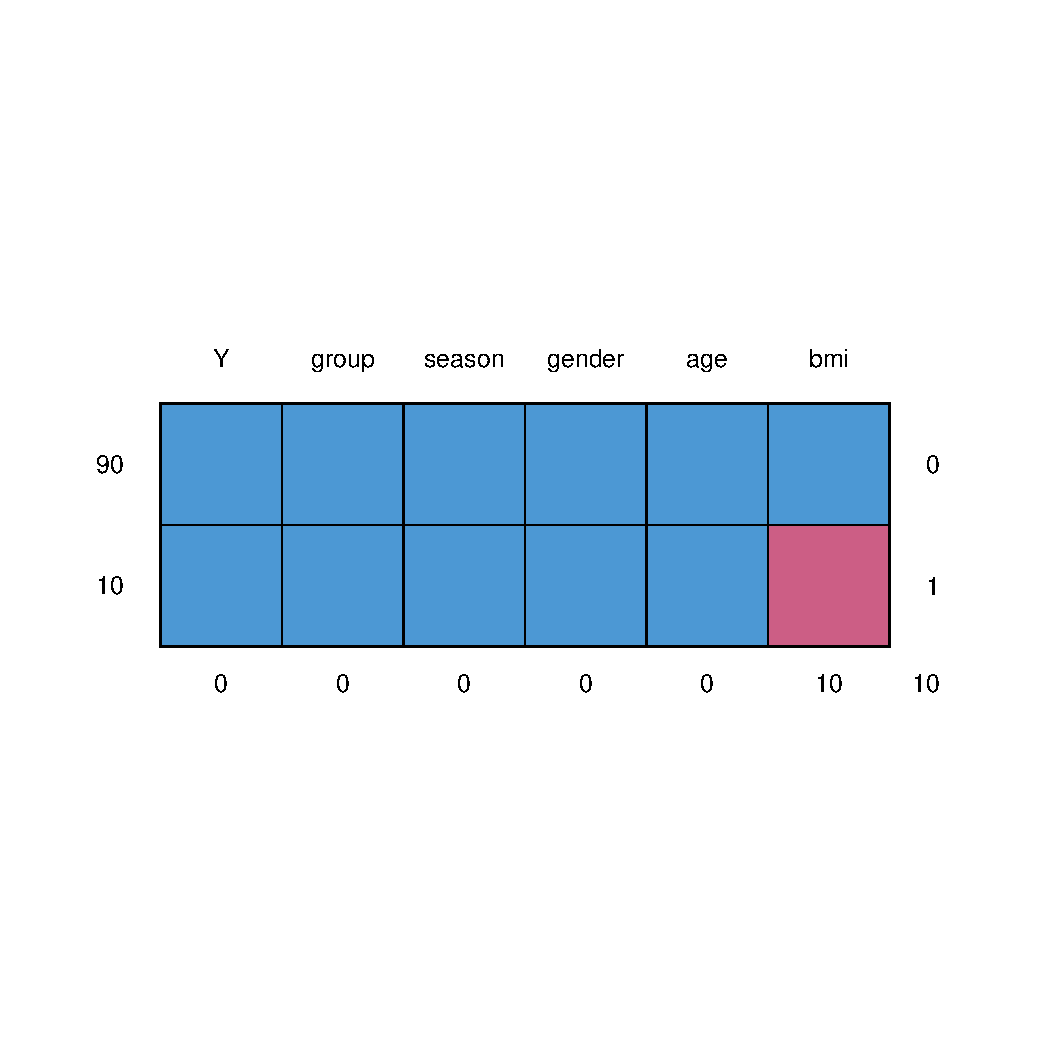
\includegraphics[width=.9\linewidth]{./figures/missingDataPattern.pdf}
\end{center}

\vspace{-4cm}

Note: with more patterns it becomes clear that the left column counts
the number of observations with a specific patern. The right column
display the index of the pattern. The bottom row counts the number of
missing value relative to each variable (and the total number of
missing values).
\lstset{language=r,label= ,caption= ,captionpos=b,numbers=none}
\begin{lstlisting}
dt.data2 <- copy(dt.data)
dt.data2[5:10,age:=NA]
md.pattern(dt.data2)
\end{lstlisting}

\begin{verbatim}
   Y group season gender age bmi   
90 1     1      1      1   1   1  0
4  1     1      1      1   1   0  1
6  1     1      1      1   0   0  2
   0     0      0      0   6  10 16
\end{verbatim}

\clearpage

\subsection{Step 2: Define imputation model}
\label{sec:orga4503bb}

\lstset{language=r,label= ,caption= ,captionpos=b,numbers=none}
\begin{lstlisting}
all.variables <- c("Y","group","season","bmi","gender","age")
n.variables <- length(all.variables)
Mlink <- matrix(0, n.variables, n.variables,
		dimnames = list(all.variables,all.variables))
Mlink["bmi",c("group","season","gender","age")] <- 1
Mlink
\end{lstlisting}

\begin{verbatim}
       Y group season bmi gender age
Y      0     0      0   0      0   0
group  0     0      0   0      0   0
season 0     0      0   0      0   0
bmi    0     1      1   0      1   1
gender 0     0      0   0      0   0
age    0     0      0   0      0   0
\end{verbatim}

A value of 1 means that the column variable is used as a predictor for
 the target block (in the rows).

\clearpage

\subsection{Step 3: Generate imputed datasets}
\label{sec:orgb3c5893}
Generate imputed values
\lstset{language=r,label= ,caption= ,captionpos=b,numbers=none}
\begin{lstlisting}
n.imputed <- 3 ## number of imputed datasets
dt.mice <- mice(dt.data,
		m=n.imputed, 
		maxit = 50, # number of iterations to obtain the imputed dataset
		predictorMatrix = Mlink,
		method = 'pmm', # Predictive mean matching, only ok for continuous variables, it is possible to set constrains for positive variables
		seed = 500, printFlag = FALSE)
summary(dt.mice)
\end{lstlisting}

\begin{verbatim}
Class: mids
Number of multiple imputations:  3 
Imputation methods:
     Y  group season    bmi gender    age 
    ""     ""     ""  "pmm"     ""     "" 
PredictorMatrix:
       Y group season bmi gender age
Y      0     0      0   0      0   0
group  0     0      0   0      0   0
season 0     0      0   0      0   0
bmi    0     1      1   0      1   1
gender 0     0      0   0      0   0
age    0     0      0   0      0   0
\end{verbatim}

\subsubsection{Interacting with the mice object}
\label{sec:org7575e2e}

Missingness indicator:
\lstset{language=r,label= ,caption= ,captionpos=b,numbers=none}
\begin{lstlisting}
table(cci(dt.mice))
\end{lstlisting}

\begin{verbatim}

FALSE  TRUE 
   10    90
\end{verbatim}


Complete case dataset:
\lstset{language=r,label= ,caption= ,captionpos=b,numbers=none}
\begin{lstlisting}
str(cc(dt.mice))
\end{lstlisting}

\begin{verbatim}
'data.frame':	90 obs. of  6 variables:
 $ Y     : num  102 82.9 94.9 61.4 82 ...
 $ group : Factor w/ 2 levels "SAD","HC": 1 2 1 1 2 2 2 2 2 2 ...
 $ season: Factor w/ 2 levels "winter","summer": 2 2 1 1 2 1 2 1 1 1 ...
 $ bmi   : num  21.6 21.9 20.6 26.4 28.5 ...
 $ gender: Factor w/ 2 levels "Male","Female": 2 2 2 1 1 2 2 1 2 2 ...
 $ age   : num  77.3 57.2 73.6 34 50.7 ...
\end{verbatim}

Extract observations with missing values:
\lstset{language=r,label= ,caption= ,captionpos=b,numbers=none}
\begin{lstlisting}
str(ic(dt.mice))
\end{lstlisting}

\begin{verbatim}
'data.frame':	10 obs. of  6 variables:
 $ Y     : num  92.2 91 63.1 76.2 75.2 ...
 $ group : Factor w/ 2 levels "SAD","HC": 1 2 1 2 1 2 2 1 2 2
 $ season: Factor w/ 2 levels "winter","summer": 2 2 2 2 1 2 2 1 1 1
 $ bmi   : num  NA NA NA NA NA NA NA NA NA NA
 $ gender: Factor w/ 2 levels "Male","Female": 2 2 1 2 2 2 1 2 1 1
 $ age   : num  68.5 62.6 34.9 50.6 54.1 ...
\end{verbatim}

Dataset after multiple imputation:
\lstset{language=r,label= ,caption= ,captionpos=b,numbers=none}
\begin{lstlisting}
str(complete(dt.mice, action = 1)) ## first imputed dataset
\end{lstlisting}

\begin{verbatim}
'data.frame':	100 obs. of  6 variables:
 $ Y     : num  92.2 91 63.1 76.2 75.2 ...
 $ group : Factor w/ 2 levels "SAD","HC": 1 2 1 2 1 2 2 1 2 2 ...
 $ season: Factor w/ 2 levels "winter","summer": 2 2 2 2 1 2 2 1 1 1 ...
 $ bmi   : num  25.9 21 16.7 20.2 25.9 ...
 $ gender: Factor w/ 2 levels "Male","Female": 2 2 1 2 2 2 1 2 1 1 ...
 $ age   : num  68.5 62.6 34.9 50.6 54.1 ...
\end{verbatim}

\lstset{language=r,label= ,caption= ,captionpos=b,numbers=none}
\begin{lstlisting}
str(complete(dt.mice, action = 2)) ## second imputed dataset
\end{lstlisting}

\begin{verbatim}
'data.frame':	100 obs. of  6 variables:
 $ Y     : num  92.2 91 63.1 76.2 75.2 ...
 $ group : Factor w/ 2 levels "SAD","HC": 1 2 1 2 1 2 2 1 2 2 ...
 $ season: Factor w/ 2 levels "winter","summer": 2 2 2 2 1 2 2 1 1 1 ...
 $ bmi   : num  17.5 18.1 24.3 20.7 20.9 ...
 $ gender: Factor w/ 2 levels "Male","Female": 2 2 1 2 2 2 1 2 1 1 ...
 $ age   : num  68.5 62.6 34.9 50.6 54.1 ...
\end{verbatim}

\clearpage

\subsection{Step 4: Check the imputed datasets}
\label{sec:orgbdb2fb4}
\subsubsection{Convergence of the imputation algorithm}
\label{sec:org5076bca}

\lstset{language=r,label= ,caption= ,captionpos=b,numbers=none}
\begin{lstlisting}
plot(dt.mice, layout = c(1,2))
\end{lstlisting}

\begin{center}
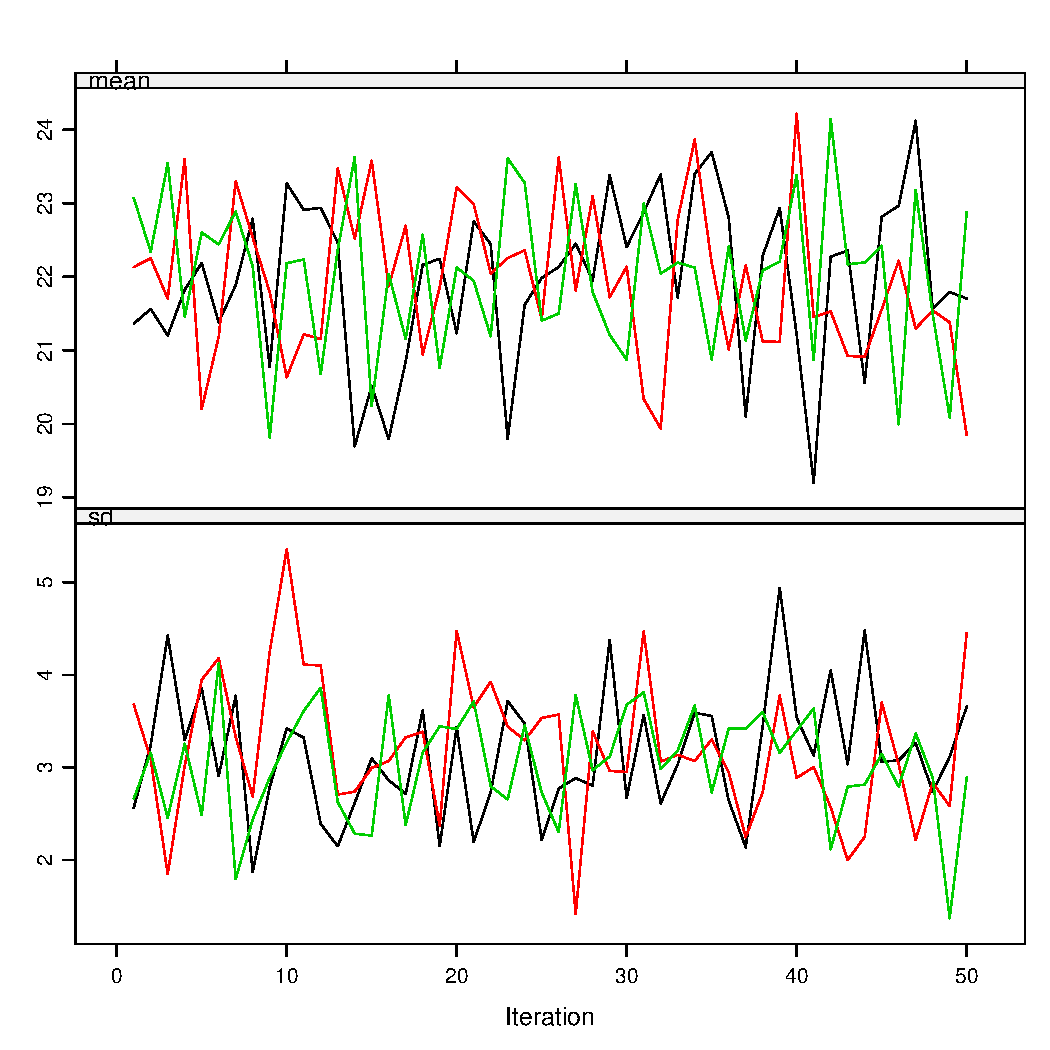
\includegraphics[width=0.70\textwidth]{./figures/traceCVimputed.pdf}
\end{center}


\subsubsection{Visualizing the imputed values}
\label{sec:org9da41d7}
Visualize imputed value values and check they are plausible (e.g. mice
is not imputed a BMI of 75):
\lstset{language=r,label= ,caption= ,captionpos=b,numbers=none}
\begin{lstlisting}
dt.mice$imp$bmi
\end{lstlisting}

\begin{verbatim}
          1        2        3
1  25.86170 17.51962 26.03528
2  20.97076 18.12224 21.60139
3  16.68404 24.25679 17.86661
4  20.15124 20.71567 26.03528
5  25.86170 20.92015 25.24236
6  24.80171 25.02219 20.62111
7  21.42336 25.02219 25.02219
8  21.00639 20.90548 20.15124
9  24.76365 12.99571 24.80171
10 15.52519 12.99571 21.42336
\end{verbatim}

The rows correspond to the 3 different imputed datasets and the
columns to 10 imputed values per dataset. One can also summarizes the
imputed values computing their quantiles:

\lstset{language=r,label= ,caption= ,captionpos=b,numbers=none}
\begin{lstlisting}
apply(dt.mice$imp$bmi,2,quantile)
\end{lstlisting}

\begin{verbatim}
            1        2        3
0%   15.52519 12.99571 17.86661
25%  20.35612 17.67028 20.82167
50%  21.21487 20.81058 23.20155
75%  24.79219 23.42263 25.18731
100% 25.86170 25.02219 26.03528
\end{verbatim}

Boxplot of the imputed values:

\lstset{language=r,label= ,caption= ,captionpos=b,numbers=none}
\begin{lstlisting}
boxplot(dt.mice$imp$bmi)
\end{lstlisting}

\begin{center}
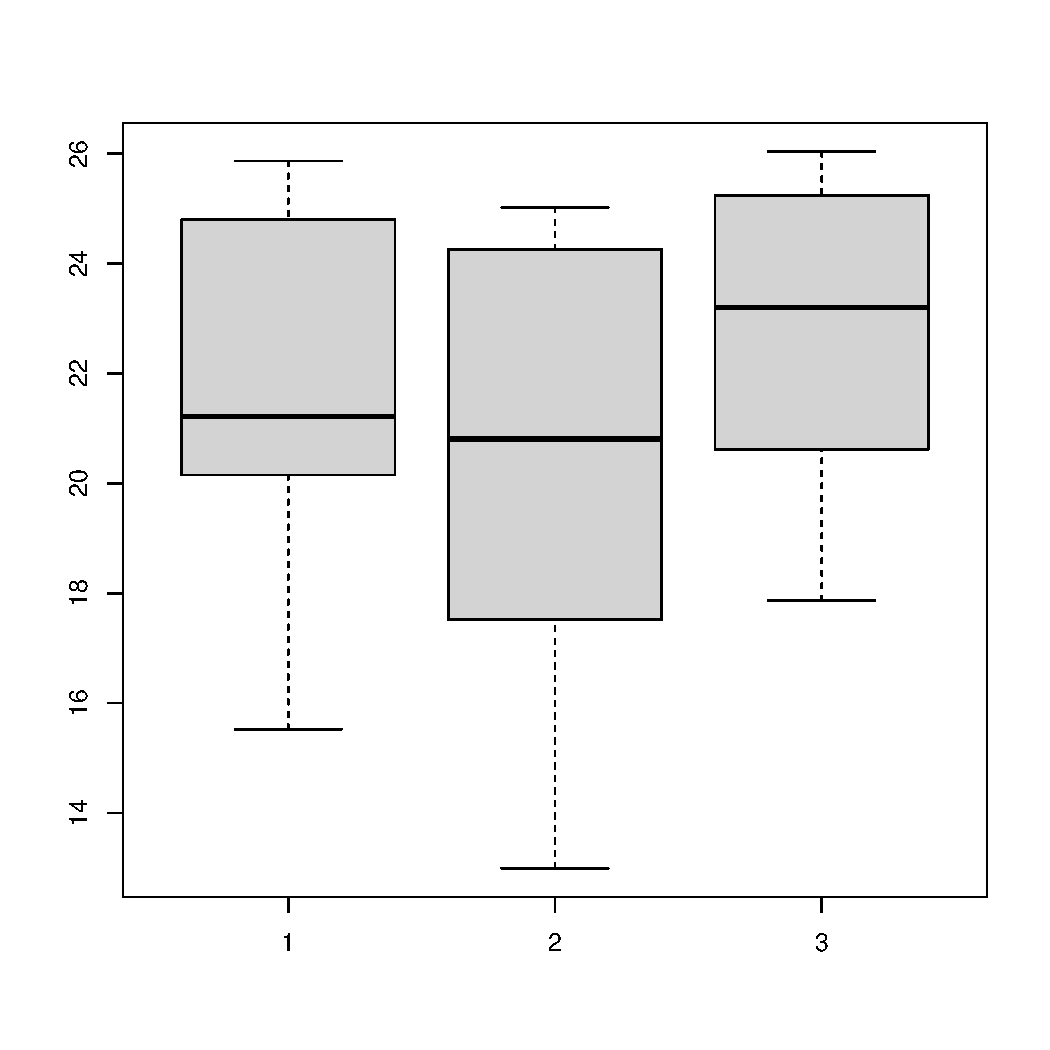
\includegraphics[width=.9\linewidth]{./figures/boxplotImputed.pdf}
\end{center}

\clearpage

Imputed values vs. observed values
\lstset{language=r,label= ,caption= ,captionpos=b,numbers=none}
\begin{lstlisting}
dt.bmi <- rbind(data.table(bmi = unlist(dt.mice$imp$bmi), imputed = TRUE),
		data.table(bmi = na.omit(dt.data$bmi), imputed = FALSE))
\end{lstlisting}

Histogram
\lstset{language=r,label= ,caption= ,captionpos=b,numbers=none}
\begin{lstlisting}
gg1.bmi <- ggplot(dt.bmi, aes(bmi, group = imputed, fill = imputed))
gg1.bmi <- gg1.bmi + geom_histogram(aes(y=..count../sum(..count..)),position = "dodge")
gg1.bmi
\end{lstlisting}

\begin{verbatim}
`stat_bin()` using `bins = 30`. Pick better value with `binwidth`.
\end{verbatim}

\begin{center}
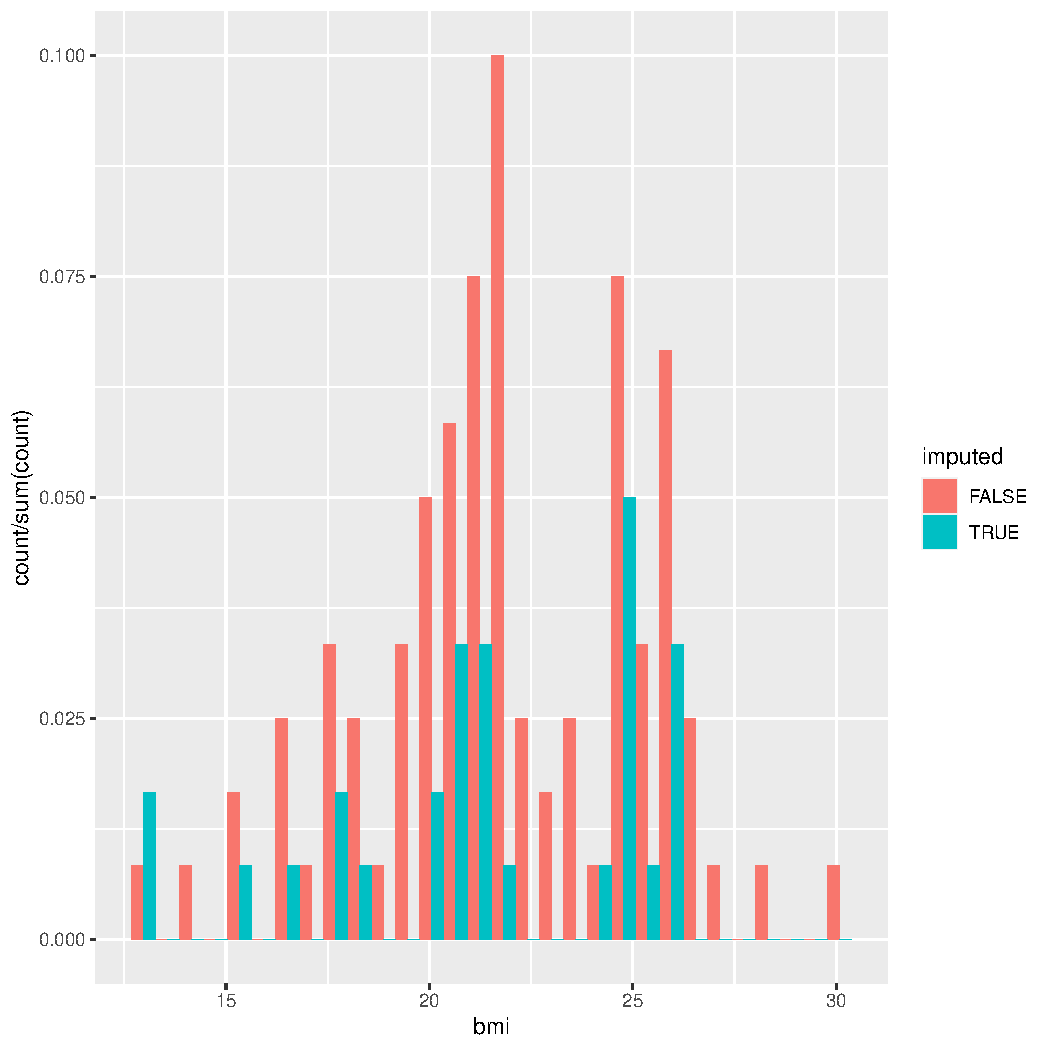
\includegraphics[width=.9\linewidth]{./figures/histImputed.pdf}
\end{center}

\clearpage

One more plot:

\lstset{language=r,label= ,caption= ,captionpos=b,numbers=none}
\begin{lstlisting}
stripplot(dt.mice, bmi~.imp, pch=20, cex=2)
\end{lstlisting}

\begin{center}
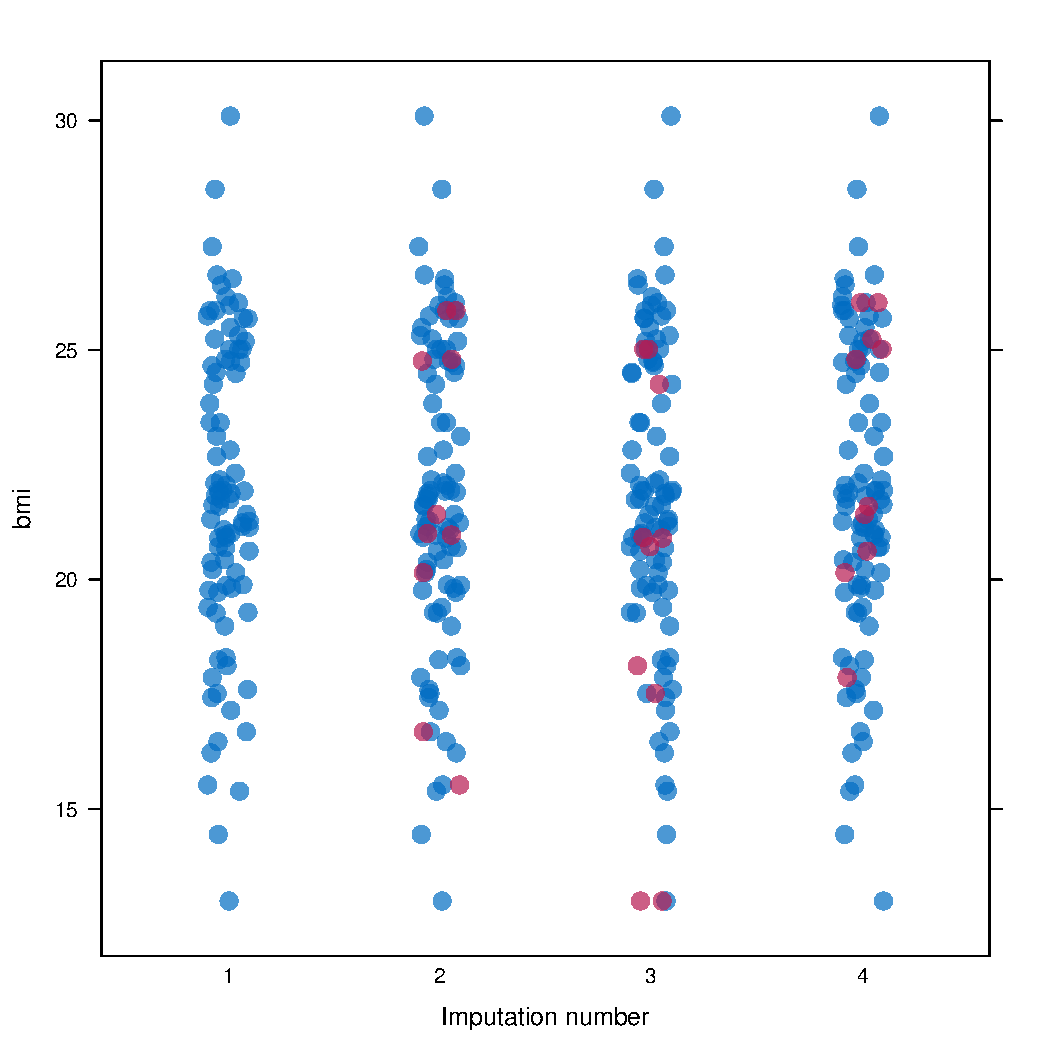
\includegraphics[width=.9\linewidth]{./figures/striplotImputed.pdf}
\end{center}

\clearpage

\subsection{Step 3: Fit the statical model on each imputed dataset}
\label{sec:orgb1d7d91}

\lstset{language=r,label= ,caption= ,captionpos=b,numbers=none}
\begin{lstlisting}
e.mice <- with(data = dt.mice,
	       lm(Y~group+season+bmi+gender+age)
	       )
e.mice
\end{lstlisting}

\begin{verbatim}
call :
with.mids(data = dt.mice, expr = lm(Y ~ group + season + bmi + 
    gender + age))

call1 :
mice(data = dt.data, m = n.imputed, method = "pmm", predictorMatrix = Mlink, 
    maxit = 50, printFlag = FALSE, seed = 500)

nmis :
     Y  group season    bmi gender    age 
     0      0      0     10      0      0 

analyses :
[[1]]

Call:
lm(formula = Y ~ group + season + bmi + gender + age)

Coefficients:
 (Intercept)       groupHC  seasonsummer           bmi  genderFemale           age  
      2.8846        0.7238        1.2174        0.8602        0.5507        1.0058  


[[2]]

Call:
lm(formula = Y ~ group + season + bmi + gender + age)

Coefficients:
 (Intercept)       groupHC  seasonsummer           bmi  genderFemale           age  
      3.8365        0.6732        0.8917        0.7907        0.7422        1.0221  


[[3]]

Call:
lm(formula = Y ~ group + season + bmi + gender + age)

Coefficients:
 (Intercept)       groupHC  seasonsummer           bmi  genderFemale           age  
      2.2639        0.5601        1.1779        0.8919        0.7209        1.0025
\end{verbatim}

We can check that using \texttt{with} is equivalent to run the linear
regression on the imputed dataset:
\lstset{language=r,label= ,caption= ,captionpos=b,numbers=none}
\begin{lstlisting}
dt.tempo <- copy(dt.data)
dt.tempo[is.na(bmi), bmi := dt.mice$imp$bmi[,1]]
lm(Y ~ group + season + bmi + gender + age, data  = dt.tempo)
\end{lstlisting}

\begin{verbatim}

Call:
lm(formula = Y ~ group + season + bmi + gender + age, data = dt.tempo)

Coefficients:
 (Intercept)       groupHC  seasonsummer           bmi  genderFemale           age  
      2.8846        0.7238        1.2174        0.8602        0.5507        1.0058
\end{verbatim}

\clearpage

\subsection{Step 4: Pool the results over the imputed datasets}
\label{sec:org4f3576a}

\lstset{language=r,label= ,caption= ,captionpos=b,numbers=none}
\begin{lstlisting}
ePool.mice <- pool(e.mice)
summary(ePool.mice)
\end{lstlisting}

\begin{verbatim}
          term  estimate  std.error statistic        df      p.value
1  (Intercept) 2.9949755 1.73919838  1.722044 18.777429 1.014936e-01
2      groupHC 0.6523698 0.42434760  1.537348 78.067966 1.282516e-01
3 seasonsummer 1.0956572 0.46036133  2.379994 30.027026 2.386256e-02
4          bmi 0.8475895 0.08552179  9.910802  7.101823 2.060982e-05
5 genderFemale 0.6712684 0.42707145  1.571794 66.444876 1.207484e-01
6          age 1.0101585 0.01664369 60.693193  6.176972 8.221885e-10
\end{verbatim}


The (pooled) estimate is the average of the estimates relative to each
imputed dataset:
\lstset{language=r,label= ,caption= ,captionpos=b,numbers=none}
\begin{lstlisting}
Q.coef <- colMeans(do.call(rbind,lapply(e.mice$analyses, coef)))
Q.coef
\end{lstlisting}

\begin{verbatim}
(Intercept)      groupHC seasonsummer          bmi genderFemale          age 
  2.9949755    0.6523698    1.0956572    0.8475895    0.6712684    1.0101585
\end{verbatim}

The variance is a bit more complex and involves:
\begin{itemize}
\item the within-imputation variance (depends on the sample size)
\end{itemize}
\lstset{language=r,label= ,caption= ,captionpos=b,numbers=none}
\begin{lstlisting}
covW <- Reduce("+",lapply(e.mice$analyses, vcov))/n.imputed
print(covW, digits = 5)
\end{lstlisting}

\begin{verbatim}
             (Intercept)     groupHC seasonsummer         bmi genderFemale         age
(Intercept)    2.1882899 -0.13040004  -0.04842230 -7.9278e-02  -0.10952359 -5.2588e-03
groupHC       -0.1304000  0.17070925   0.01361091  3.0162e-03   0.00655971 -6.6906e-04
seasonsummer  -0.0484223  0.01361091   0.16981498 -2.3136e-03   0.01559623 -2.0107e-04
bmi           -0.0792775  0.00301620  -0.00231365  3.7376e-03  -0.00042973 -4.6547e-05
genderFemale  -0.1095236  0.00655971   0.01559623 -4.2973e-04   0.16771404  2.9411e-04
age           -0.0052588 -0.00066906  -0.00020107 -4.6547e-05   0.00029411  1.3100e-04
\end{verbatim}

\begin{itemize}
\item the between-imputation variance (depends on the amount of missing data)
\end{itemize}
\lstset{language=r,label= ,caption= ,captionpos=b,numbers=none}
\begin{lstlisting}
ls.diffCoef <- lapply(e.mice$analyses, function(iI){coef(iI)-Q.coef})
covB <- Reduce("+",lapply(ls.diffCoef,tcrossprod))/(n.imputed-1)
print(covB, digits = 5)
\end{lstlisting}

\begin{verbatim}
           [,1]        [,2]       [,3]        [,4]        [,5]        [,6]
[1,]  0.6273908  0.03854326 -0.1225940 -0.04085088  0.01833254  0.00804290
[2,]  0.0385433  0.00702122 -0.0015717 -0.00218666 -0.00585420  0.00032147
[3,] -0.1225940 -0.00157170  0.0315882  0.00839604 -0.01252242 -0.00179271
[4,] -0.0408509 -0.00218666  0.0083960  0.00268231 -0.00167818 -0.00053567
[5,]  0.0183325 -0.00585420 -0.0125224 -0.00167818  0.01100699  0.00049399
[6,]  0.0080429  0.00032147 -0.0017927 -0.00053567  0.00049399  0.00010951
\end{verbatim}

\begin{itemize}
\item the simulation error
\end{itemize}
\lstset{language=r,label= ,caption= ,captionpos=b,numbers=none}
\begin{lstlisting}
covE <- covB/n.imputed
print(covE, digits = 5)
\end{lstlisting}

\begin{verbatim}
           [,1]        [,2]        [,3]        [,4]        [,5]        [,6]
[1,]  0.2091303  0.01284775 -0.04086467 -0.01361696  0.00611085  2.6810e-03
[2,]  0.0128478  0.00234041 -0.00052390 -0.00072889 -0.00195140  1.0716e-04
[3,] -0.0408647 -0.00052390  0.01052939  0.00279868 -0.00417414 -5.9757e-04
[4,] -0.0136170 -0.00072889  0.00279868  0.00089410 -0.00055939 -1.7856e-04
[5,]  0.0061108 -0.00195140 -0.00417414 -0.00055939  0.00366900  1.6466e-04
[6,]  0.0026810  0.00010716 -0.00059757 -0.00017856  0.00016466  3.6504e-05
\end{verbatim}

The total variance is:
\lstset{language=r,label= ,caption= ,captionpos=b,numbers=none}
\begin{lstlisting}
covT <- covW + covB + covE
\end{lstlisting}

leading to the standard errors:
\lstset{language=r,label= ,caption= ,captionpos=b,numbers=none}
\begin{lstlisting}
sqrt(diag(covT))
\end{lstlisting}
\begin{verbatim}
(Intercept)      groupHC seasonsummer          bmi genderFemale          age 
 1.73919838   0.42434760   0.46036133   0.08552179   0.42707145   0.01664369
\end{verbatim}


\bigskip

There is also a function to extract the R-squared:
\lstset{language=r,label= ,caption= ,captionpos=b,numbers=none}
\begin{lstlisting}
pool.r.squared(e.mice)
\end{lstlisting}

\begin{verbatim}
          est     lo 95     hi 95 fmi
R^2 0.9890535 0.9819615 0.9933666 NaN
\end{verbatim}

\lstset{language=r,label= ,caption= ,captionpos=b,numbers=none}
\begin{lstlisting}
vec.rsquared <- sapply(e.mice$analyses, function(iImp){
    summary(iImp)$r.squared
})
tanh(mean(atanh(vec.rsquared)))
\end{lstlisting}

\begin{verbatim}
[1] 0.9890535
\end{verbatim}

\clearpage

\section{Special case: imputation using a specific law and no covariate}
\label{sec:org663d68f}
Mice can be adapted in order, for instance, to sample from a uniform
distribution or a truncated normal distribution. First define a
function able to generate data like:
\lstset{language=r,label= ,caption= ,captionpos=b,numbers=none}
\begin{lstlisting}
mice.impute.SI_unif <- function(y, ry, ...){ ## uniform law
    n.NA <- sum(ry==FALSE)
    sample <- runif(n.NA, min = 0, max = 1)
    return(cbind(sample))
}
\end{lstlisting}

or

\lstset{language=r,label= ,caption= ,captionpos=b,numbers=none}
\begin{lstlisting}
mice.impute.SI_tnorm <- function(y, ry, ...){ ## truncated normal law
    require(truncnorm)
    n.NA <- sum(ry==FALSE)
    sample <- rtruncnorm(n.NA, a = 0, b = 1, mean = 1, sd = 0.1)
    return(cbind(sample))
}
\end{lstlisting}
Then prepare the matrix indicating which variable should be used
during the imputation:
\lstset{language=r,label= ,caption= ,captionpos=b,numbers=none}
\begin{lstlisting}
impute.var <- c("bmi","group")
Mlink2 <- matrix(0, 
		 nrow = length(impute.var), 
		 ncol = length(impute.var), 
		 dimnames = list(impute.var,impute.var))
Mlink2["bmi","group"] <- 1
Mlink2
\end{lstlisting}

\begin{verbatim}
      bmi group
bmi     0     1
group   0     0
\end{verbatim}

\clearpage 

Then run mice as usual except that the method should correspond to one of the previous functions:
\lstset{language=r,label= ,caption= ,captionpos=b,numbers=none}
\begin{lstlisting}
n.imputed <- 50 ## number of imputed datasets
set.seed(1)
dt.mice2 <- mice(dt.data,
		 m=n.imputed, 
		 maxit = 1, # not relevant
		 predictorMatrix = Mlink2, # not relevant
		 method = 'SI_tnorm', # function previous define (without "mice.impute.")
		 seed = 500, printFlag = FALSE)
\end{lstlisting}

Then as usual one should check that the imputed values are satisfying:
\lstset{language=r,label= ,caption= ,captionpos=b,numbers=none}
\begin{lstlisting}
quantile(unlist(dt.mice2$imp$bmi))
\end{lstlisting}

\begin{verbatim}
       0%       25%       50%       75%      100% 
0.7041556 0.8790477 0.9317021 0.9687630 0.9997288
\end{verbatim}


\lstset{language=r,label= ,caption= ,captionpos=b,numbers=none}
\begin{lstlisting}
hist(unlist(dt.mice2$imp$bmi))
\end{lstlisting}

\begin{center}
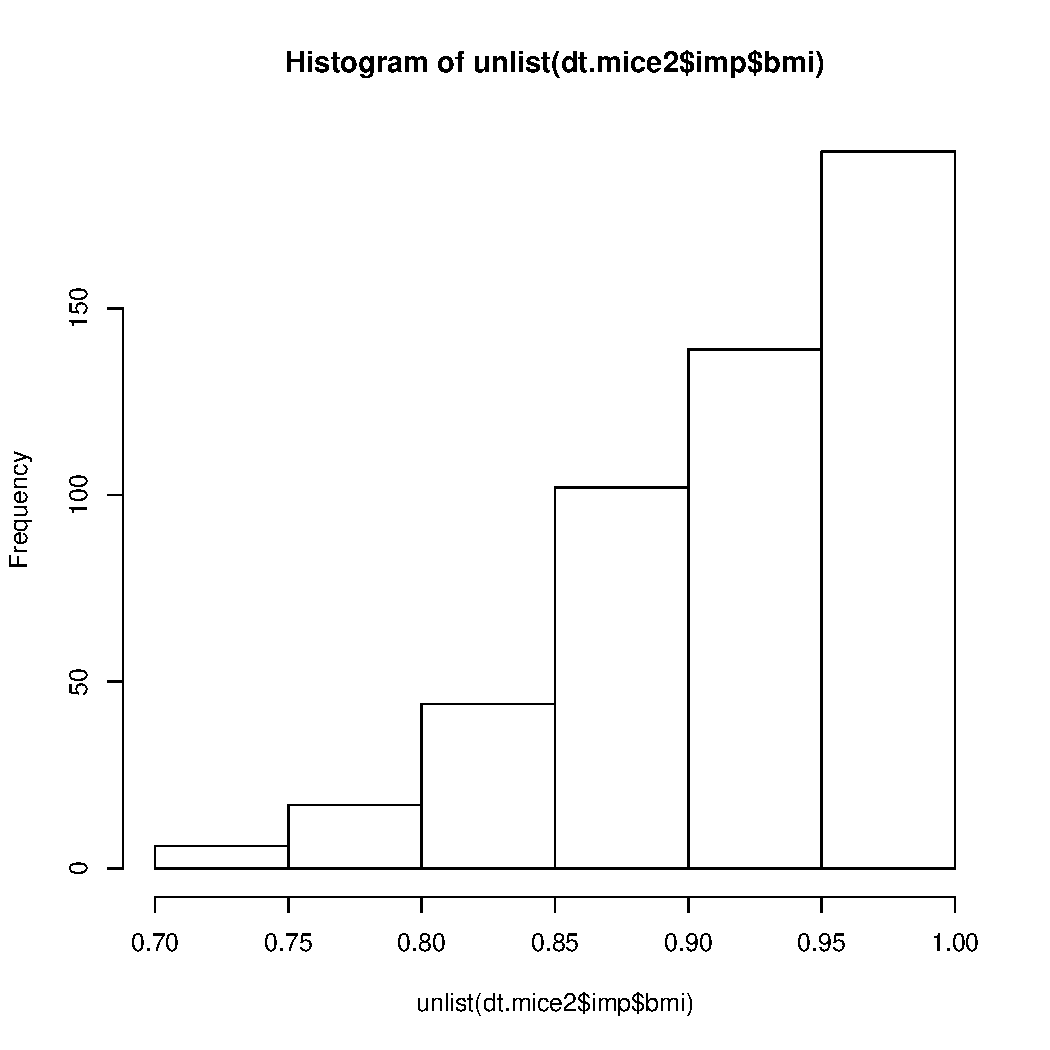
\includegraphics[width=0.8\textwidth]{./figures/histImputed2.pdf}
\end{center}

\clearpage

One more plot:
\lstset{language=r,label= ,caption= ,captionpos=b,numbers=none}
\begin{lstlisting}
stripplot(dt.mice2, bmi~.imp, pch=20, cex=2)
\end{lstlisting}

\begin{center}
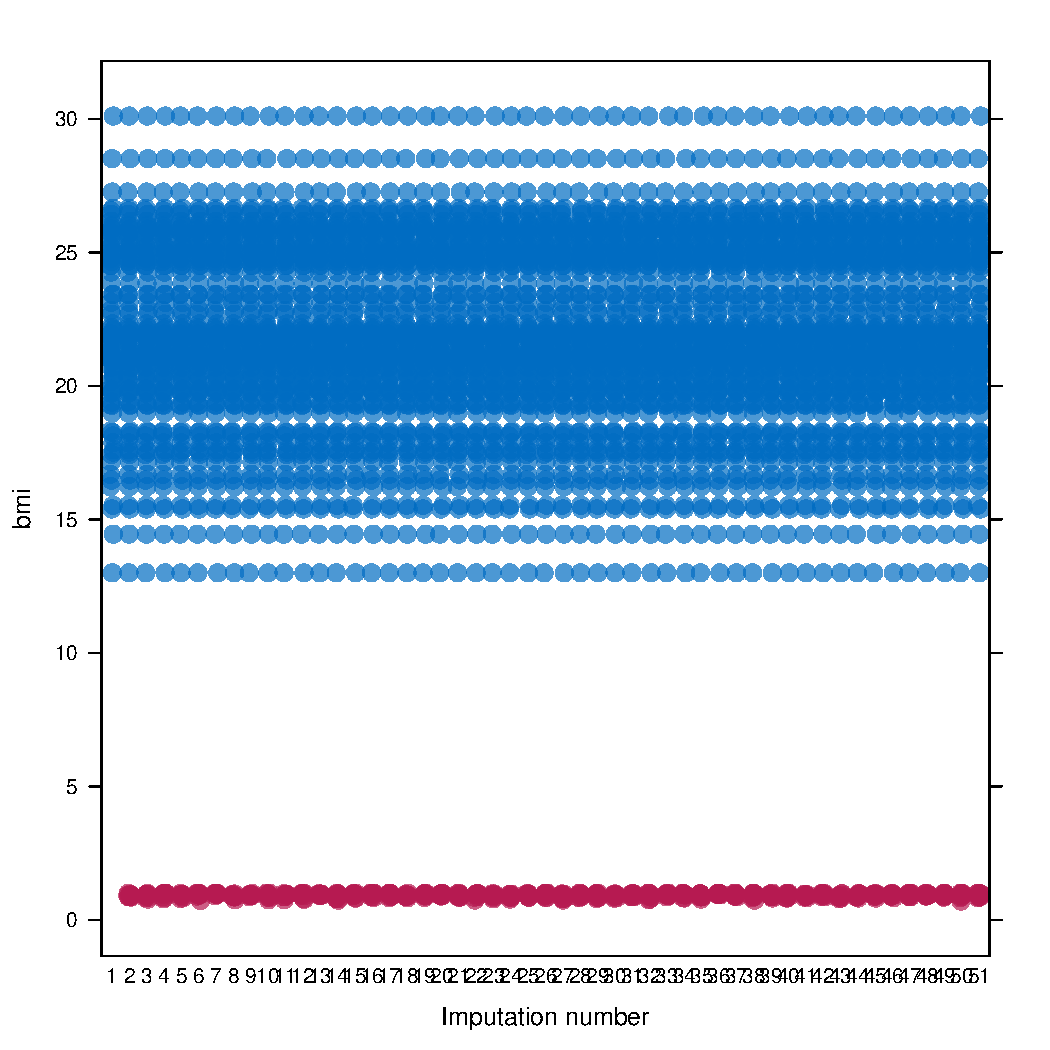
\includegraphics[width=.9\linewidth]{./figures/striplotImputed2.pdf}
\end{center}

Here for instance the imputed values does not overlap the observed one
so something (i.e. the parameters of the distribution used for the
imputation) is wrong.

\clearpage

\section{Reporting guideline}
\label{sec:org3a3313b}
From \url{https://stefvanbuuren.name/Winnipeg/Lectures/Winnipeg.pdf}:
\begin{itemize}
\item Amount of missing data
\item Reasons for missingness
\item Differences between complete and incomplete data
\item Method used to account for missing data
\item Software
\item Number of imputed datasets
\item Imputation model
\item Derived variables
\item Diagnostics
\item Pooling
\item Listwise deletion
\item Sensitivity analysis
\end{itemize}
\end{document}